
%%%%%%%%%%%%%%%%%%%%%%%%%%%%%%%%%%%%%%%%%%%%%%%%%%%%%%%%%%%%%%%%%%%%%%%%
%
%		LINEAR ALGEBRA
%
%%%%%%%%%%%%%%%%%%%%%%%%%%%%%%%%%%%%%%%%%%%%%%%%%%%%%%%%%%%%%%%%%%%%%%%%


\begin{topic}[Linear Algebra]

\end{topic}


\newpage


\begin{module}
	\Title{Linear Combinations}

	\Heading{Textbook} Section 1.1

	\Heading{Objectives}
	\begin{itemize}
		\item Internalize vectors as geometric objects representing displacements.

		\item Use column vector notation to write vectors.

		\item Relate points an vectors and be able to interpret a point as
			a vector and a vector as a point.

		\item Solve simple equations involving vectors.
	\end{itemize}

	\Heading{Motivation} Students have differing levels of experience with vectors.
	We want to establish a common notation for vectors and use vector notation
	along with algebra to solve simple questions. E.g., ``How can I get to location
	$A$ given that I can only walk parallel to the lines $y=4x$ and $y=-x$?''


	\begin{annotation}
		\begin{notes}
			\begin{itemize}
			\item
			We will use the language \emph{component of $\vec v$ in
			the direction $\vec u$} in the future and it will be a \emph{vector}.
			For this reason, try to refer to the entries of a column
			vector as \emph{coordinates} or \emph{entries} instead of components.

			\item
			Though we will almost exclusively use
			column vector notation in this course, students should be able to parse
			questions phrased in terms of row vectors.
			\end{itemize}
		\end{notes}
	\end{annotation}
	
	We will use column vector notation and the idea of equating
	coordinates in order to solve problems.

\end{module}


\section*{Task 1.1: The Magic Carpet Ride}
\addcontentsline{toc}{subsection}{Task 1.1: The Magic Carpet Ride}


\begin{annotation}
	\begin{goals}
		\Goal{Hands-on experience with vectors as displacements.}
		\begin{itemize}
			\item Internalize vectors as geometric objects representing
				displacements.

			\item Use column vector notation to write vectors.

			\item Use pre-existing knowledge of algebra to answer vector
				questions.
		\end{itemize}
	\end{goals}
	\begin{notes}

		\begin{itemize}
			\item There are many ways to solve this problem.
				Some students
				might start with equations. After they use their
				equations to solve the problem, make them draw a picture
				and come up with a graphical solution.

			\item When the students start coming up with vector equations,
				give them the vocabulary of \emph{linear
				combinations}
				and \emph{column vector notation}.
		\end{itemize}
	\end{notes}
\end{annotation}
You are a young traveler, leaving home for the first time. Your parents
want to help you on your journey, so just before your departure, they give you two
gifts. Specifically, they give you two forms of transportation: a hover board and
a magic carpet. Your parents inform you that both the hover board and the magic carpet
have restrictions in how they operate:

\begin{minipage}{\textwidth}
	\vspace{.5cm}
	\begin{wrapfigure}{l}{1in}
	\vspace{-.8cm}
	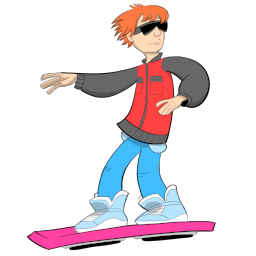
\includegraphics[width=1in]{images/HoverBoard-small.png}
	\end{wrapfigure}

	We denote the restriction on the hover board's movement by the vector
	$\mat{3 \\1}$. By this we mean that if
	the hover board traveled ``forward'' for one hour, it would move along a
	``diagonal'' path that would result in a displacement of 3 miles East and
	1 mile North of its starting location.
\end{minipage}

\begin{minipage}{\textwidth}
	\vspace{.5cm}
	\begin{wrapfigure}{l}{1in}
	\vspace{-.8cm}
	
\includegraphics[width=1in]{images/MagicCarpet-small.png}
	\end{wrapfigure}

	We denote the restriction on the magic carpet's movement by the vector
	$\mat{1 \\2 }$. By this we mean that if the
	magic carpet traveled ``forward'' for one hour, it would move along a
	``diagonal'' path that would result in a displacement of 1 mile East and
	2 miles North of its starting location.
\end{minipage}

\lfoot{\footnotesize Drawings by \url{@DavidsonJohnR} (twitter)}

\vspace{10mm}

% Scenario Section
\textbf{Scenario One: The Maiden Voyage}

Your Uncle Cramer suggests that your first adventure should be to go visit
the wise man, Old Man Gauss. Uncle Cramer tells you that Old Man Gauss
lives in a cabin that is 107 miles East and 64 miles North of your home.

\vspace{5mm}

\textbf{Task:}
\par
Investigate whether or not you can use the hover board and the magic
carpet to get to Gauss's cabin. If so, how? If it is not possible to
get to the cabin with these modes of transportation, why is that the case?

%\vspace{5mm}
% As a group, state and explain your answer(s) on the group whiteboard. Use
% the vector notation for each mode of transportation as part of your
% explanation and use a diagram or graphic to help illustrate your
% point(s).


\begin{module}
	\Title{Linear Combinations}

	\Heading{Textbook}
	Section 1.2

	\Heading{Objectives}
	\begin{itemize}
		\item Set up and solve vector equations $a\vec v+b\vec u=\vec w$. The solving
			method may be ad hoc.
		\item Use set notation and set operations/relations $\cup$, $\cap$, $\in$, $\subseteq$.
		\item Translate between set-builder notation and words in multiple ways.
	\end{itemize}

	\Heading{Motivation}
	We revisit questions about linear combinations more formally and generate a need for
	algebra. The algebra we do to solve vector equations will become algorithmic when
	we learn row reduction, but at the moment, any method is fine.

	\begin{annotation}
		\begin{notes}
			You will have a mix of MAT135/136 and MAT137 students.
			The MAT137 students will be doing logic and sets in their
			class. The MAT135 students won't. Make sure not to leave them
			behind!
		\end{notes}
	\end{annotation}
	As we talk about more complex objects, we need precise ways to talk about
	groups of vectors. I.e., we need sets and set-builder notation. This preview of set-builder
	notation will take some of difficulty away when we define span as a set of vectors.

	In this course we will be using formal and precise language. Part of this module
	is that there are multiple correct ways (and multiple incorrect ways) to use formal
	language. Gone are the days of ``there's only one right answer and it is 4''!

\end{module}


\section*{Task 1.2: The Magic Carpet Ride, Hide and Seek}
\addcontentsline{toc}{subsection}{Task 1.2: The Magic Carpet Ride, Hide and Seek}


\begin{annotation}
	\begin{goals}
		\Goal{Address an existential question involving vectors: ``Is it possible
		to find a linear combination that does\ldots?''}

		The goal of this problem is to
		\begin{itemize}
			\item Formalize geometric questions using the language of vectors.
			\item Find both geometric and algebraic arguments to support the same
				conclusion.
			\item Establish what a ``negative multiple'' of a vector should be.
		\end{itemize}
	\end{goals}
	\begin{notes}
		\begin{itemize}
			\item Both \emph{yes} and \emph{no} are valid answers to
				this question depending on whether you are allowed
				to go backwards. Establish that ``negative'' multiples of
				a vector mean traveling backwards along that vector.
			\item This problem can be solved with algebra by finding a formula
				for the coefficients for an arbitrary position or with geometry,
				with arguments eventually hinging on the fact that non-parallel
				lines do not intersect.
		\end{itemize}
	\end{notes}
\end{annotation}
You are a young traveler, leaving home for the first time. Your parents
want to help you on your journey, so just before your departure, they give
you two gifts. Specifically, they give you two forms of transportation:
a hover board and a magic carpet. Your parents inform you that both the
hover board and the magic carpet have restrictions in how they operate:



\begin{minipage}{\textwidth}
	\vspace{.5cm}
	\begin{wrapfigure}{l}{1in}
	\vspace{-.8cm}
	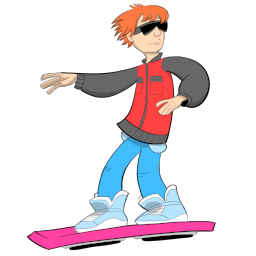
\includegraphics[width=1in]{images/HoverBoard-small.png}
	\end{wrapfigure}

	We denote the restriction on the hover board's movement by the vector
	$\mat{3 \\1}$. By this we mean that if
	the hover board traveled ``forward'' for one hour, it would move along a
	``diagonal'' path that would result in a displacement of 3 miles East and
	1 mile North of its starting location.
\end{minipage}

\begin{minipage}{\textwidth}
	\vspace{.5cm}
	\begin{wrapfigure}{l}{1in}
	\vspace{-.8cm}
	
\includegraphics[width=1in]{images/MagicCarpet-small.png}
	\end{wrapfigure}

	We denote the restriction on the magic carpet's movement by the vector
	$\mat{1 \\2 }$. By this we mean that if the
	magic carpet traveled ``forward'' for one hour, it would move along a
	``diagonal'' path that would result in a displacement of 1 mile East and
	2 miles North of its starting location.
	\vspace{1cm}
\end{minipage}



\textbf{Scenario Two: Hide-and-Seek}

Old Man Gauss wants to move to a cabin in a different location. You are
not sure whether Gauss is just trying to test your wits at finding him
or if he actually wants to hide somewhere that you can't visit him.

\vspace{5mm}

\textbf{Are there some locations that he can hide and you cannot reach him
with these two modes of transportation?}

Describe the places that you
can reach using a combination of the hover board and the magic carpet and
those you cannot. Specify these geometrically and algebraically. Include
a symbolic representation using vector notation. Also, include a convincing
argument supporting your answer.

%\vspace{5mm} \par \textbf{Use your
%group's whiteboard as a space to write out our work as your work together
%on this problem.}



\pagestyle{siefken}

\section*{Sets and Set Notation}
\vspace{-.5cm}

	\begin{definition}[Set]
		A \emph{set} is a (possibly infinite) collection of items
		and is notated with curly braces (for example, $\{1,2,3\}$ is
		the set containing the numbers 1, 2, and 3).  We call the items in
		a set \emph{elements}.

		If $X$ is a set and $a$ is an element of $X$, we may write $a\in X$,
		which is read ``$a$ is an element of $X$.''

		If $X$ is a set, a \emph{subset} $Y$ of $X$ (written $Y\subseteq X$)
		is a set such that every element of $Y$ is an element of $X$. Two sets are
		called \emph{equal} if they are subsets of each other (i.e., $X=Y$ if
		$X\subseteq Y$ and $Y\subseteq X$).

		We can define a subset using \emph{set-builder notation}.
		That is, if $X$ is a set, we can define the subset
		\[
			Y= \Set*{a\in X \given \text{some rule involving }a},
		\]
		which is read ``$Y$ is the set of $a$ in $X$ {\bf such that} some rule
		involving $a$ is true.''  If $X$ is intuitive, we may omit it and
		simply write $Y=\{a:\text{some rule involving }a\}$.  You may equivalently
		use ``$|$'' instead of ``$:$'', writing $Y=\{a\,|\,\text{some rule involving }a\}$.
	\end{definition}

	\begin{definition}
		Some common sets are
		\begin{itemize}
			\item[] $\N=\Set{\text{natural numbers}} = \Set{\text{non-negative whole numbers}}$.
			\item[] $\Z=\Set{\text{integers}} = \Set{\text{whole numbers, including negatives}}$.
			\item[] $\R=\Set{\text{real numbers}}$.
			\item[] $\R^n=\Set{\text{vectors in $n$-dimensional Euclidean space}}$.
		\end{itemize}
	\end{definition}


	\question
	\begin{annotation}
		\begin{goals}
			\Goal{Practice reading sets and set-builder notation.}

			The goal of this problem is to
			\begin{itemize}
				\item Become familiar with $\in$, $\subseteq$, and $=$ in
					the context of sets.
				\item Distinguish between $\in$ and $\subseteq$.
				\item Use quantifiers with sets.
			\end{itemize}
		\end{goals}

		\begin{notes}
			\begin{itemize}
				\item Most are easy up through (h).
				\item Make students ``fix'' (i) so it
					becomes true.
				\item (j) and (k) are an opportunity to use
					the definition of set equality. Students don't
					realize that $=$'s has a definition.
			\end{itemize}
		\end{notes}
	\end{annotation}
	\begin{parts}
		\item Which of the following statements are true?
		\begin{enumerate}
			\item $3\in\Set{1,2,3}$.
				\begin{solution}[inline]True\end{solution}
			\item $1.5\in\Set{1,2,3}$.
				\begin{solution}[inline]False\end{solution}
			\item $4\in\Set{1,2,3}$.
				\begin{solution}[inline]False\end{solution}
			\item ``b''$\in \Set{ x \given x\text{ is an English letter}}$.
				\begin{solution}[inline]True\end{solution}
			\item ``\`o''$\in \Set{x \given x\text{ is an English letter}}$.
				\begin{solution}[inline]False\end{solution}
			\item $\Set{1,2} \subseteq \Set{1,2,3}$.
				\begin{solution}[inline]True\end{solution}
			\item For some $a\in \Set{1,2,3}$, $a \geq 3$.
				\begin{solution}[inline]True\end{solution}
			\item For any $a\in \Set{1,2,3}$, $a\geq 3$.
				\begin{solution}[inline]False\end{solution}
			\item $1 \subseteq \Set{1,2,3}$.
				\begin{solution}[inline]False\end{solution}
			\item $\Set{1,2,3}=\Set{x\in\R \given 1\leq x\leq 3}$.
				\begin{solution}[inline]False\end{solution}
			\item $\Set{1,2,3}=\Set{x\in\Z \given 1\leq x\leq 3}$.
				\begin{solution}[inline]True\end{solution}
		\end{enumerate}
	\end{parts}

	\question
	\begin{annotation}
		\begin{goals}
			\Goal{Practice writing sets using set-builder notation.}

			The goal of this problem is to
			\begin{itemize}
				\item Express English descriptions using math notation.
				\item Recognize there is more than one correct way to
					write formal math.
				\item Preview vector form of a line.
			\end{itemize}
		\end{goals}

		\begin{notes}
			\begin{itemize}
				\item There are multiple correct ways to write
					each of these sets. It's a good opportunity
					to get man correct and incorrect sets up on the
					board for discussing.
				\item Don't worry about the geometry of $B$. That's coming
					in a later problem.
			\end{itemize}
		\end{notes}
	\end{annotation}
		Write the following in set-builder notation
	\begin{parts}
			\item The subset $A\subseteq \R$ of real numbers larger than $\sqrt{2}$.
				\begin{solution}
					$\Set*{x\in\R \given x>\sqrt{2}}$.
				\end{solution}
			\item The subset $B\subseteq \R^2$ of vectors whose first coordinate
			is twice the second.
				\begin{solution}
					$\Set*{\vec v\in\R^2\given \vec v=\mat{a\\b}\text{ with }a=2b}$
					or
					$\Set*{\vec v\in\R^2\given\vec v=\mat{2t\\t}\text{ for some }t\in \R}$\\
					or
					$\Set*{\mat{a\\b}\in\R^2\given a=2b}$.
				\end{solution}
	\end{parts}

	\begin{definition}[Unions \& Intersections]
		Two common set operations are \emph{unions} and \emph{intersections}.
		Let $X$ and $Y$ be sets.

		\hfill\begin{minipage}{\dimexpr\textwidth-3cm}
		\begin{itemize}
			\item[(union)] $X\cup Y = \Set{ a \given a\in X\text{ or }a\in Y}$.
			\item[(intersection)] $X\cap Y = \Set{ a \given a\in X\text{ and }a\in Y}$.
		\end{itemize}
		\end{minipage}
	\end{definition}

	\question
	\begin{annotation}
		\begin{goals}
			\Goal{Apply the definition of $\cup$ and $\cap$.}
		\end{goals}

		\begin{notes}
			\begin{itemize}
				\item It's not important to emphasize that $\cup$ and $\cap$ are binary
			operations but we ask for $X\cup Y\cup Z$ without parenthesis.
			Students won't worry if you don't bring it up.
				\item It won't be clear to them how to write the empty set.
					Some will write $\{\emptyset\}$. Make sure this comes out.
			\end{itemize}
		\end{notes}
	\end{annotation}
	Let $X=\Set{1,2,3}$ and $Y=\Set{2,3,4,5}$ and $Z=\Set{4,5,6}$.  Compute
	\begin{parts}
		\item $X\cup Y$ \begin{solution}[inline]$\Set{1,2,3,4,5}$\end{solution}
		\item $X\cap Y$ \begin{solution}[inline]$\Set{2,3}$\end{solution}
		\item $X\cup Y\cup Z$ \begin{solution}[inline]$\Set{1,2,3,4,5,6}$\end{solution}
		\item $X\cap Y\cap Z$ \begin{solution}[inline]$\emptyset=\Set{}$\end{solution}
	\end{parts}


\begin{module}
	\Title{Visualizing Sets, Formal Language of Linear Combinations}

	\Heading{Textbook}
	Section 1.2

	\Heading{Objectives}
	\begin{itemize}
		\item Draw pictures of formally-described subsets of $\R^2$.
		\item Graphically represent $\cup$ and $\cap$ for subsets of $\R^2$.
		\item Graphically represent linear combinations and then come up with
			algebraic arguments to support graphical intuition.
	\end{itemize}

	\Heading{Motivation}

	We want to build a bridge between the formal language of linear combinations
	and set-builder notation and geometric intuition. Where as last time
	the focus was on formal language, this time the focus is on linking geometry
	to formal descriptions.


\end{module}

	\question
	\begin{annotation}
		\begin{goals}
			\Goal{Visualize sets of vectors.}

			The goal of this problem is to
			\begin{itemize}
				\item Apply set-builder notation in the context of vectors.
				\item Distinguish between ``for all'' and ``for some''
					in set builder notation.
				\item Practice unions and intersections.
				\item Practice thinking about set equality.
			\end{itemize}
		\end{goals}

		\begin{notes}
			\begin{itemize}
				\item 1--3 will be easy.
				\item Have a discussion about when you
					should draw vectors as arrows
					vs\mbox{.} as points.
				\item 4 gets at a subtle point that will come up again
					when we define span.
				\item Many will miss 7. Writing a proof for this is
					good practice.
			\end{itemize}
		\end{notes}
	\end{annotation}
	Draw the following subsets of $\R^2$.
	\begin{parts}
		\item $V=\Set*{\vec x\in\R^2 \given \vec x=\mat{0\\t}\text{ for some }t\in\R}$.
		\item $H=\Set*{\vec x\in\R^2 \given \vec x=\mat{t\\0}\text{ for some }t\in\R}$.
		\item $D=\Set*{\vec x\in\R^2 \given \vec x=t\mat{1\\1}\text{ for some }t\in\R}$.
		\begin{solution}
	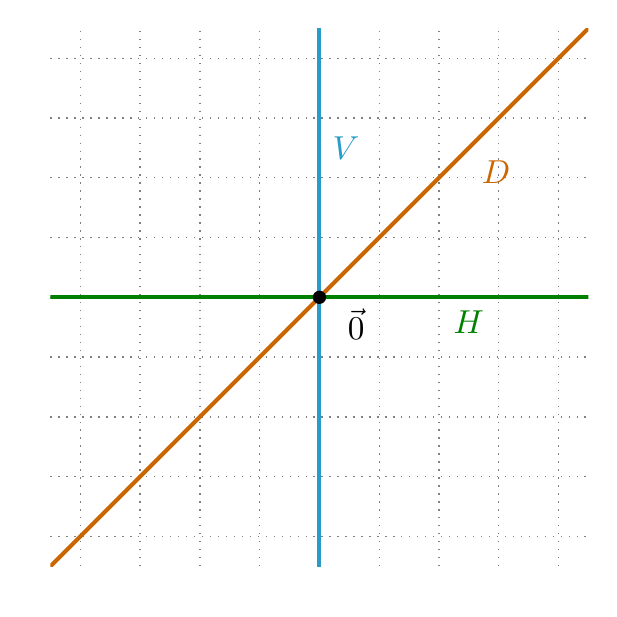
\begin{tikzpicture}[scale=1.2, >=latex]
    \begin{axis}[scale=1,
		    axis equal image,
		    axis line style={draw=none},
		    tick style={draw=none},
		    yticklabels={,,},
		    xticklabels={,,},
		 xmin=-4.5,
		 xmax=4.5,
		 ymin=-4.5,
		 ymax=4.5,
		 major grid style={dotted, gray},
                 xtick={-10,-9,...,10},
                 ytick={-10,-9,...,10},
                 grid=both,
		 anchor=origin]

	    \draw[Green, very thick] (-5,0) -- (5,0) node[near end, below] {$H$};
	    \draw[cyan!80!black, very thick] (0,-5) -- (0,5) node[near end, right] {$V$};
	    \draw[orange!80!black, very thick] (-5,-5) -- (5,5) node[near end, below right] {$D$};

	    \fill[fill=black] (0,0) circle[radius=2pt] node[below right, xshift=5pt] {\color{black}$\vec 0$};
    \end{axis}
\end{tikzpicture}
		\end{solution}
		\item $N=\Set*{\vec x\in\R^2 \given \vec x=t\mat{1\\1}\text{ for all }t\in\R}$.
				\begin{solution}[inline]
			$N=\Set{}$.
		\end{solution}

		\item $V\cup H$.
			\begin{solution}[inline]
			$V\cup H$ looks like a ``$+$'' going through the origin.
		\end{solution}
		\item $V\cap H$.
			\begin{solution}[inline]
				$V\cap H=\Set{\vec 0}$ is just the origin.
		\end{solution}
		\item Does $V\cup H=\R^2$?
			\begin{solution}
				No. $V\cup H$ does not contain $\mat{1\\1}$ while $\R^2$ does contain
				$\mat{1\\1}$.
			\end{solution}
	\end{parts}

\section*{Vector Combinations}
	\vspace{-1em}

	\begin{definition}[Linear Combination]
		A \emph{linear combination} of the vectors $\vec v_1,\vec v_2,\ldots,\vec v_n$ is
		a vector
		\[
			\vec w = \alpha_1\vec v_1+\alpha_2\vec v_2+\cdots+\alpha_n\vec v_n.
		\]
		The scalars $\alpha_1,\alpha_2,\ldots,\alpha_n$ are called the \emph{coefficients} of the linear combination.
	\end{definition}

	\question
	\label{ProbSkewBasis}
	\begin{annotation}
		\begin{goals}
			\Goal{Practice linear combinations.}

			The goal of this problem is to
			\begin{itemize}
				\item Practice using the formal term \emph{linear combination}.
				\item Foreshadow span.
			\end{itemize}
		\end{goals}

		\begin{notes}
			\begin{itemize}
				\item In 2, the question should arise: ``Is $3\vec v_1$
					a linear combination of $\vec v_1$ \emph{and}
					$\vec v_2$?'' Address this.
				\item Refer to the magic carpet ride for 5. You don't
					need to do a full proof.
			\end{itemize}
		\end{notes}
	\end{annotation}
	Let $\vec v_1=\mat{1\\1}$, $\vec v_2=\mat{1\\-1}$, and $\vec w=2\vec v_1+\vec v_2$.
	\begin{parts}
		\item Write $\vec w$ as a column vector. When $\vec w$ is written as a
			linear combination of $\vec v_1$ and $\vec v_2$, what are the
			coefficients of $\vec v_1$ and $\vec v_2$?
			\begin{solution}
				$\vec w=\mat{3\\2}$; the coefficients are $(2,1)$.
			\end{solution}
		\item Is $\mat{3\\3}$ a linear combination of $\vec v_1$ and $\vec v_2$?
			\begin{solution}[inline]
				Yes. $\mat{3\\3}=3\vec v_1+0\vec v_2$.
			\end{solution}

		\item Is $\mat{0\\0}$ a linear combination of $\vec v_1$ and $\vec v_2$?
			\begin{solution}[inline]
				Yes. $\vec 0=0\vec v_1+0\vec v_2$.
			\end{solution}
		\item Is $\mat{4\\0}$ a linear combination of $\vec v_1$ and $\vec v_2$?
			\begin{solution}[inline]
				Yes. $\mat{4\\0}=2\vec v_1+2\vec v_2$.
			\end{solution}
		\item Can you find a vector in $\R^2$ that isn't a linear combination of
		$\vec v_1$ and $\vec v_2$?
			\begin{solution}
				No. $\mat{1\\0}=\tfrac{1}{2}\vec v_1+\tfrac{1}{2}\vec v_2$ and
				$\mat{0\\1}=\tfrac{1}{2}\vec v_1-\tfrac{1}{2}\vec v_2$.
				Therefore
				\[
					\mat{a\\b}
					= a\mat{1\\0}+b\mat{0\\1}
					= a(\tfrac{1}{2}\vec v_1+\tfrac{1}{2}\vec v_2)
						+b(\tfrac{1}{2}\vec v_1-\tfrac{1}{2}\vec v_2)
					=(\tfrac{a+b}{2})\vec v_1+(\tfrac{a-b}{2})\vec v_2.
				\]
				Therefore any vector in $\R^2$ can be written as linear combinations
				of $\vec v_1$ and $\vec v_2$.
			\end{solution}
		\item Can you find a vector in $\R^2$ that isn't a linear combination of
			$\vec v_1$?
			\begin{solution}
				Yes. All linear combinations of $\vec v_1$ have equal $x$ and
				$y$ coordinates, therefore $\vec w=\mat{2\\1}$ is not a linear
				combination of $\vec v_1$.
			\end{solution}
	\end{parts}


	\question
	\begin{annotation}
		\begin{goals}
			\Goal{Practice formal writing.}
		\end{goals}

		\begin{notes}
			\begin{itemize}
				\item Make everyone \emph{write}. They will think
					they can do it, but they will find it hard if
					they try.
			\end{itemize}
		\end{notes}
	\end{annotation}
	Recall the \emph{Magic Carpet Ride} task where the hover board could
	travel in the direction $\vec h=\mat{3\\1}$ and the magic carpet could
	move in the direction $\vec m=\mat{1\\2}$.
	\begin{parts}
		\item Rephrase the sentence \emph{``Gauss can be reached using just the
			magic carpet and the hover board''} using formal mathematical
			language.
			\begin{solution}
				Gauss's location can be written as a linear combination of
				$\vec m$ and $\vec h$.
			\end{solution}
		\item Rephrase the sentence \emph{``There is nowhere Gauss can hide
			where he is inaccessible by magic carpet and hover board''} using
			formal mathematical language.
			\begin{solution}
				Every vector in $\R^2$ can be written as a linear combination
				of $\vec m$ and	$\vec h$.
			\end{solution}
		\item Rephrase the sentence \emph{``$\R^2$ is the set of all linear
			combinations of $\vec h$ and $\vec m$''} using formal mathematical
			language.
			\begin{solution}
				$\R^2=\Set{\vec v\given \vec v=t\vec m+s\vec h\text{ for some }t,s\in \R}$.
			\end{solution}
	\end{parts}

\begin{module}
	\Title{Restricted Linear Combinations, Lines}

	\Heading{Textbook} Section 1.2

	\Heading{Objectives}
	\begin{itemize}
		\item Read and digest a new definition.

		\item Use pictures to explore a new concept.

		\item Convert from an equation-representation of a line to a set-representation.
	\end{itemize}

	\Heading{Motivation} Part of doing math in the world is reading and understanding
	other people's definitions. Most students will not have heard of non-negative
	linear combinations or convex linear combinations. This is a chance for them
	to read and try to understand these formal definitions. They will need to
	draw pictures to get an intuition about what these concepts mean.

	These concepts are useful in their own right, and in particular, convex linear
	combinations can be used to describe line segments. Adding these definitions
	to a student's toolbox serves the goal of \emph{being able to describe
	the world with mathematics}.

	To that end, we start working with lines. Lines are something students have
	used since grade school, but they worked with them in $y=mx+b$ form which
	is only applicable in $\R^{2}$. We want to convert this representation
	into vector form and set-based descriptions which apply to all
	dimensions.

\end{module}

	\displayonlynewpage
	\begin{definition}[Non-negative \& Convex Linear Combinations]
		The linear combination $\vec w=\alpha_1\vec v_1+\alpha_2\vec v_2+\cdots+\alpha_n\vec v_n$ is
		called a \emph{non-negative} linear combination of $\vec v_1,\vec v_2,\ldots,\vec v_n$ if
		$\alpha_1,\alpha_2,\ldots,\alpha_n\geq 0$.

		If $\alpha_1,\alpha_2,\ldots,\alpha_n\geq 0$
		and $\alpha_1+\alpha_2+\cdots+\alpha_n=1$, then $\vec w$ is called a \emph{convex} linear combination
	of  $\vec v_1,\vec v_2,\ldots,\vec v_n$.
	\end{definition}

	\question
	\begin{annotation}
		\begin{goals}
			\Goal{Geometric meaning of \emph{non-negative} and \emph{convex}
			linear
			combinations.}

			The goal of this problem is to
			\begin{itemize}
				\item Read and apply the definition of non-negative and convex
					linear combinations.
				\item Gain geometric intuition for non-negative and convex linear
					combinations.
				\item Learn how to describe line segments using
					convex linear combinations.
			\end{itemize}
		\end{goals}

		\begin{notes}
			\begin{itemize}
				\item This question is about reading and applying;
					emphasize that before they start.
				\item The geometry won't be obvious. Ask them to \emph{draw} specific
					linear combinations (e.g., $(1/2,1/2)$) to get an idea.
				\item They know $\vec a$ and $\vec b$ span all vectors from problem \ref{ProbSkewBasis}.
				\item In part 1, they will forget $\vec a$ and $\vec b$ are linear combinations of themselves.
				\item Part 2 (b) highlights a degeneracy that will come up again when discussing linear independence and dependence. Explain how the 
					picture for non-negative linear combinations
					almost always looks one way, but this case is an exception.
			\end{itemize}
		\end{notes}
	\end{annotation}
	Let
	\[
		\vec a=\mat{1\\1} \qquad \vec b=\mat{-1\\1}\qquad \vec c=\mat{0\\1}\qquad\vec d=\mat{0\\2}\qquad\vec e=\mat{-1\\-1}.
	\]
	\begin{parts}
		\item Out of $\vec a$, $\vec b$, $\vec c$, $\vec d$, and $\vec e$, which
			vectors are
			\begin{enumerate}
				\item linear combinations of $\vec a$ and $\vec b$?
				\begin{solution}[inline]
					All of them, since any vector in $\R^2$ can be written as a linear combination
					of $\vec a$ and $\vec b$.
				\end{solution}

				\item non-negative linear combinations of $\vec a$ and $\vec b$?
				\begin{solution}[inline]
					$\vec a$, $\vec b$, $\vec c$, $\vec d$.
				\end{solution}

				\item convex linear combinations of $\vec a$ and $\vec b$?
				\begin{solution}[inline]
					$\vec a$, $\vec b$, $\vec c$.
				\end{solution}
			\end{enumerate}

		\item If possible, find two vectors $\vec u$ and $\vec v$ so that
			\begin{enumerate}
				\item $\vec a$ and $\vec c$ are non-negative linear combinations
					of $\vec u$ and $\vec v$ but $\vec b$ is not.
				\begin{solution}
					Let $\vec u=\vec a$ and $\vec v=\vec c$.
				\end{solution}

				\item $\vec a$ and $\vec e$ are non-negative linear combinations
					of $\vec u$ and $\vec v$.
				\begin{solution}
					Let $\vec u=\vec a$ and $\vec v=\vec e$.
				\end{solution}

				\item $\vec a$ and $\vec b$ are non-negative linear combinations
					of $\vec u$ and $\vec v$ but $\vec d$ is not.
				\begin{solution}
					Impossible. If $\vec a$ and $\vec b$ are non-negative
					linear combinations of $\vec u$ and $\vec v$, then every non-negative
					linear combination of $\vec a$ and $\vec b$ is also a non-negative
					linear combination of $\vec u$ and $\vec v$. And, we already concluded that
					$\vec d$ is a non-negative linear combination of $\vec a$ and $\vec b$.
				\end{solution}

				\item $\vec a$, $\vec c$, and $\vec d$ are convex linear
					combinations of $\vec u$ and $\vec v$.
				\begin{solution}
					Impossible. Convex linear combinations all lie on the same line segment,
					but $\vec a$, $\vec c$, and $\vec d$ are not collinear.
				\end{solution}
			\end{enumerate}Otherwise, explain why it's not possible.
	\end{parts}

	\displayonlynewpage
\section*{Lines and Planes}

	\question
	\begin{annotation}
		\begin{goals}
			\Goal{Link prior knowledge to new notation/concepts.}

			The goal of this problem is to
			\begin{itemize}
				\item Convert between $y=mx+b$ form of a line and
					the set-builder definition of the same line.
				\item Think about lines in terms of vectors rather
					than equations.
			\end{itemize}
		\end{goals}

		\begin{notes}
			\begin{itemize}
				\item This question is foreshadowing for vector form of a line.
				\item In part 3, some will draw $\vec d$ from the origin and
					some will draw it on the line. Both are fine, but make
					sure they understand that $\vec d\notin L$ by the end of
					part 4.
			\end{itemize}
		\end{notes}
	\end{annotation}
	Let $L$ be the set of points $(x,y)\in\R^2$ such that $y=2x+1$.
	\begin{parts}
		\item Describe $L$ using set-builder notation.
			\begin{solution}
				$\Set*{\vec v\in\R^2 \given \vec v=\matc{t\\2t+1}\text{ for some } t\in\R}$\\
				or
				$\Set*{\mat{x\\y}\in\R^2 \given y=2x+1}$
				or
				$\Set*{\matc{t\\2t+1}\in\R^2 \given t\in\R}$
			\end{solution}
		\item Draw $L$ as a subset of $\R^2$.
		\item Add the vectors $\vec a=\mat{-1\\-1}$, $\vec b=\mat{1\\3}$ and
			$\vec d=\vec b-\vec a$ to your drawing.
			\begin{solution}
				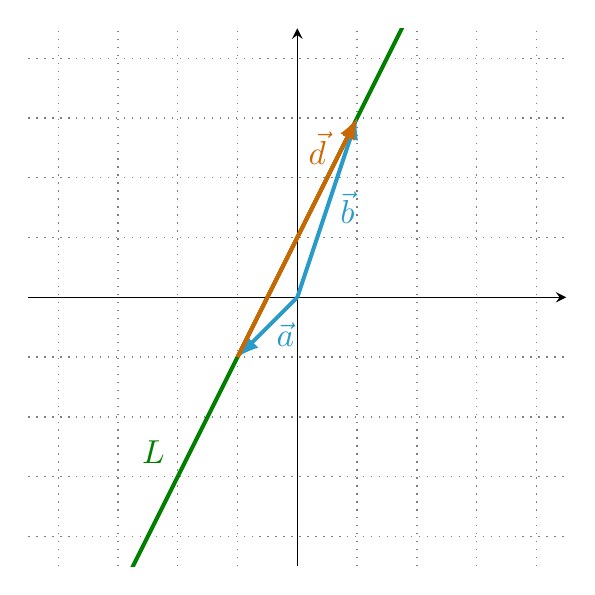
\begin{tikzpicture}[scale=1.2, >=latex]
			    \begin{axis}[scale=1,
					    axis equal image,
					    axis lines=middle,
					    axis line style = {black},
					    tick style={draw=none},
					    yticklabels={,,},
					    xticklabels={,,},
					 xmin=-4.5,
					 xmax=4.5,
					 ymin=-4.5,
					 ymax=4.5,
					 major grid style={dotted, gray},
					 xtick={-10,-9,...,10},
					 ytick={-10,-9,...,10},
					 grid=both,
					 anchor=origin]

				    \draw[Green, very thick] (-5,-9) -- (5,11) node[pos=.3, above left] {$L$};
				    \draw[cyan!80!black, very thick, ->] (0,0) -- (-1,-1) node[pos=.2, below] {$\vec a$};
				    \draw[cyan!80!black, very thick, ->] (0,0) -- (1,3) node[pos=.5, right] {$\vec b$};
				    \draw[orange!80!black, very thick, ->] (-1,-1) -- (1,3) node[near end, above, xshift=-3pt] {$\vec d$};

			    \end{axis}
				\end{tikzpicture}
			\end{solution}
		\item Is $\vec d\in L$? Explain.
			\begin{solution}
				No. $\vec d=\mat{2\\4}$ and so its entries don't satisfy $y=2x+1$.
			\end{solution}
		\item For which $t\in\R$ is it true that $\vec a+t\vec d\in L$? Explain using your picture.
			\begin{solution}
				$\vec a +t\vec d\in L$ for any $t\in \R$. We can see this because if we start at the
				vector $\vec a$ and the displace by $t\vec d$, we will always be on the line $L$.
			\end{solution}
	\end{parts}



